\documentclass[draft,12pt,oneside]{CUNY_PhD}
%%\documentclass{article}
\usepackage{graphicx}
%%\usepackage[dvips]{graphicx}
\usepackage{fixltx2e}
\usepackage[export]{adjustbox}
\usepackage{epsfig}
\graphicspath{ {./Images/} }
%%\DeclareGraphicsExtensions{.pdf,.png}
\usepackage{hyperref}
\hypersetup{
    colorlinks=true,
    linkcolor=blue,
    filecolor=magenta,      
    urlcolor=cyan,
}
\begin{document}

\pagestyle{headings}
\title{Bird Song Neuroscience Modeling}
\author{Lior Baron}  
\maketitle
Bird song neuroscience modeling – Motivation, current state and future research trends


\makeabstractpage{Advisor name}{Neural basis for bird song learning and production raises several research focus areas that help scientists better understand the underlying neural basis of complex behavior. Over the past few decades, scientists made breakthroughs in identification of the circuitry of key areas in the bird’s brain that are involved in song acquisition and production and empirical observations neural circuitry shed light into how the bird brain processes information necessary to produce the song as well as raising further questions that inspire future research. Open questions regarding the functionality of one of the key areas (HVC) involved in rhythmic aspect of song production inspire modeling that aim to explain the internal circuitry that produced stereotyped behavior observed in singing birds. This survey will cover some of the background, motivation and relevant model for bird song neural circuitry}
\tableofcontents

\mainmatter

\section*{Survey Organization}
This computational neuroscience survey covers the intersection of neuroscience and machine learning used for modeling the neurophysiological aspects of bird song. The survey begins with a brief introduction to bird song neuroscience and the motivation for using machine learning modeling. We then introduce a more detailed review of bird song neuroscience covering both song production and song acquisition brain circuitry in Chapter 2. Chapter 3 covers some modeling techniques that are used for modeling complex task and machine learning. Chapter 4 reviews some of the current models used to explain recent observations in bird song neurophysiology and help guide future research and understanding. Chapter 5 briefly summarizes the key takeaways 
\chapter{Introduction}
\section{Bird song acquisition}
According to Nottebohm, when biologists seek to understand complex system they often adopt a specific model for generalization. The idea behind is that once a model system is well understood, the model serves as foundation for further research into other species \cite{1}. Examples for generalized system methodology include the giant axon of squid is used to learn neural transmission properties, the fruit fly’s homeobox genes research helped to understand embryonic developed and sea slugs are used to study the molecular biology of learning. 
The neural mechanism of bird song can be compared to human speech acquisition as claimed by Mooney \cite{14}. Like human speech development in babies, young birds (Hatchlings) are learning to sing by first listening to song rendition by an adult member of the colony (not necessarily the parent) until they learn to recognize the mentor’s song. Later, the hatchlings start to mimic the song by first omitting babbling sounds and slowly adapting the sounds it makes to match the mentor’s song. Usually, the juvenile bird will then adapt the final song to vary slightly from the mentor’s song and thus becoming unique song in the colony.
\section{Significance of learning the neural foundations of bird song}
Brainard claims that the neural mechanism of speech development in human babies is not fully understood currently\cite{11}. Like juvenile birds, babies start to make babbling sounds few months after birth and then can take a year or more to be able to omit a complete word. In both humans and birds (along with few other species like whales, apes and others) speech acquisition is a highly complex task which require sensory input (sounds), memorization of sound sequence and fine-tuning motor output to the voice cords and lungs. An open question whether human speech and bird singing are related mechanism or parallel evolution of capabilities.
\section{Machine learning uses for modeling complex task performance}
Per LeCun, there are currently several areas in machine learning that deal with language and speech \cite{13}. Natural Language processing (NLP) is a major research area for many companies large and small (Google, Amazon, Apple and Microsoft to name few) with focus on a more natural way for humans to communicate with computers. Another area of research is in assistive technologies for the visually impaired where speaking computer (or phone) assist an individual to navigate in complex environments (like shops, streets or crowded spaces). However, in this survey, we will focus on more on the parallels between machine learning models seeking to explain neurophysiological observations. 
One of the main challenges to better understand our brain is that we can only observe very few attributes of brain activities. For years, EEG technology, which traces small electric current generated by large population of spiking neurons was the primary method to learn of brain activity. Later technologies like fMRI allowed for 3d images of brain activity to be observed but time resolution is impacted. These methods do not allow for the granular resolution of time and space needed to really understand biological network dynamics. Even late development like recording from population of neurons using light sensitive / light emitting neurons which allow for very granular time and space resolution are on a very small scale of only few neurons \cite{22}.
Machine learning can assist in understanding the inner workings of the brain in two ways. First, machine learning can help analyze large amount of noisy data collected during neuroscience experiments and researchers distilled data to for further analysis. Second, developing models of neural networks that behave similarly to biological ones can assist in further understanding of the inner working of the biological network.
\chapter{Neuroscience of bird song}
The discovery of discrete brain structures in the oscine brain that take part in song production and learning has allowed for progress in understanding how the bird’s brain supports song production. One of the earliest experiments by Nottebohm et al. involved lesioning different parts of the bird brain and then observing the behavior of birds post lesion procedure \cite{12}. Nottebohm et al. were able to carefully analyze the results from both bird behavior and neural pathology to pinpoint the borders areas involved in song learning and production, along with connectivity to other areas involved in song acquisition. 
\begin{figure}[h]
\centering
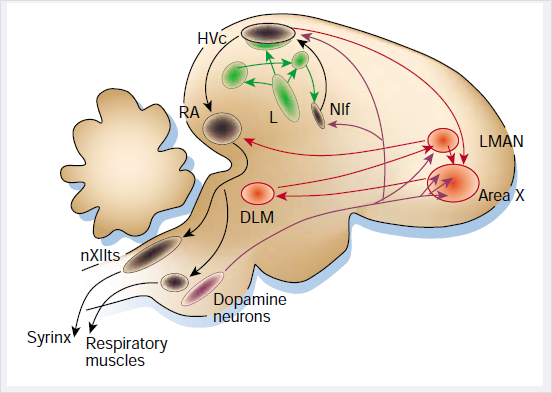
\includegraphics[scale=0.3]{Map}
\caption{Key areas and pathways involved in bird song acquisition and production - From \cite{11}}\label{Fig 1}
\end{figure}
The discovery of Song Motor Pathway (SMP) highlighted in black above and the Anterior Forebrain pathway (in red) laid the foundations for further investigation of the role played by each specialized area and how the entire pathway integrates neural signaling into very precise and stereotyped motor input required for repeated song production. Both pathways (SMP and AFP) are organized in hierarchy where the HVC area is where song production and acquisition neural signaling originates.


\section{Song production neuroscience}
Along the SMP, the HVC to RA neurons display a very stereotyped behavior where only one HVC\textsubscript{RA} neuron is active in any given time during bird song production. When active HVC\textsubscript{RA} neurons are firing at a very high rate (+200Hz) for a short period and then become inactive (while the next HVC\textsubscript{RA} neuron is active). The nature of the timely precise and sparse HVC\textsubscript{RA} firing is not fully known, and current research is seeking to understand the neural mechanism of HVC using both physiological observation and computational modelling. 
The next part of SMP involves RA  Motor neurons that are involved in song production (Syrinx and raspatory muscles). The RA pre-motor area provides continuous input to the motor muscles throughout the entire song duration and research by Leonardo et al. \cite{4} has shown that multiple HVC\textsubscript{RA} neurons are converging on single RA neuron ensemble. Another important observation is that same song syllable repeated later in song motif sequence will include one RA ensemble but different ensembles of HVC\textsubscript{RA} neurons activity.

\section{Song acquisition neuroscience}
The neurophysiological foundations of song learning are yet to be fully understood. Progress was made by \cite{12} to identify key areas along the AFP that area involved in the song acquisition process by showing that lesioning areas (like area X, LMAN or HVC) disabled or severely impacted song learning. In addition, there are areas outside traditional AFP areas that are necessary for song learning. For example, auditory feedback is necessary for song acquisition in two ways. First, the young bird needs to hear the tutor song to memorize it during the initial few weeks, and second – auditory feedback is needed to adapt the babbling sounds to match the memorized tutor song. Research by Brainard has shown that deafening birds after they memorized the tutor song but before song fully acquired resulted stopped the song acquisition process and the bird was unable to acquire the song \cite{11}. In addition, in the same study Brainard demonstrated that auditory feedback was shown to be not critical for mature song production post acquisition \cite{11}.
An open question regarding the function of the key areas identified along the AFP and their support of song acquisition and production remains open. The first stop along the pathway is HVC\textsubscript{x} neurons in the avian basal ganglia. Observations by Markowitz et al. on the type of input that HVC\textsubscript{x} neurons pass to area X and these neurons do not display the stereotypical sparse firing over time observed in HVC\textsubscript{RA} neurons of birds with crystalized songs \cite{9}. HVC\textsubscript{x} neurons seem to pass a more random tonic input to Area X and recording from HVC by Markowitz et al. showed that HVC\textsubscript{x} neurons fire anti-phase correlation with interneurons at about 30Hz and correlated within 100 nm (e.g. co activation of HVC\textsubscript{x} neurons spans 100nm or less) \cite{9}. From area X, the next stops along the AFP are the DLM area in the avian thalamus and then the LMAN area in the basal ganglia. From there, LMAN\textsubscript{RA} neurons integrate the signal back to the RA\textsubscript{Motor neurons} to produce song syllables. Studies of LMAN by Aronov et al. have shown that LMAN\textsubscript{RA} neurons are involved in babbling sound production during early phase of juvenile birds’ song learning and their input is characterized by activation that is correlated with sound production during the early babbling phase \cite{6}. However, the correlation of activity does not display the stereotyped sparse activation of HVC\textsubscript{RA} neurons. Further, Aronov et al. has shown that the HVC is not needed to produce the juvenile subsong babbling in young hatchlings (less than 45 days post hatching - dph) and the lesioning of HVC did not cause the bird to be silent during this early phase of song development \cite{6}. 

\chapter{Neural networks models}
To better understand the inner workings and dynamics of key areas along the SMP and AFP pathways, scientists like Fiete, Leonardo and Fee \cite{2}\cite{3}\cite{5} develop computational models that address gaps in understanding of neurons connectivity, interaction and signal integration. The need for computational models arise from the fact that although brain researchers have many tools these days to conduct their research (like electrophysiological recordings, fMRI, calcium imaging etc.), the information available to research tends to be sparse and noisy. Computational models allow scientist to validate models based on research findings and identify new targets for research to validate models’ assumptions.
With the advancements in machine learning over the past 20 years, researchers have few basic models from which they can develop computational models for simulations. Artificial Neural Networks have been used for many years to recognize data patterns or classify observations into categories.
\section{Convolutional networks}
According to LeCun et al. the current state of the art methodology is machine learning using Convolutional Networks that like the brain structure in some areas, uses multiple feed forward layers of artificial neurons to calculate output based on input and integrate signals between layers as the calculation moves forward deeper in the network until the last layer of the network produces the output \cite{13}. 
Although Convolutional networks are used in both academia and industry to perform machine learning, there are some key differences between how a deep learning network acquire and produce output in comparison to a biological network. 
First, Convolutional network use a process called “back propagation” to adjust connection strength between upstream and downstream neurons during the learning phase of the network based on prediction error. The magnitude of the correction in weight in each learning iteration depends on the output error in the last output layer of the network. Biologically, there is no known mechanism that relay back a distant output to each synapse along a neuronal pathway when adapting network connections strength. 
In addition, there are many other differences between the deep network model and biologically feasible networks. These include learning that requires many tagged samples for training of deep networks, the mathematical functions that maps input to output and the assumption on the organization of deep feed forward network, which might not occur at all at the brain region in question. 
\section{Recurrent neural networks (RNNs)}
Another candidate network for modeling that LeCun reviews at \cite{13} is a recurrent neural network (RNN) in which the neurons are connected not in a feed forward manner but receive input from neighboring neurons and even self-input from previous time step. There are few flavors of RNNs that are used for different tasks including natural language processing and videos. RNNs process the input sequentially and each unit receive the input from the previous layer / units from step t-1 (including its own output at step t-1) and calculates an output based on the weighted input. Like deep networks, RNNs use back propagation to adjust the input weights when the network makes a prediction error during training. Unlike deep network, the back-propagation process can be very long since the network contains circular paths and requires special consideration and assumption when using back propagation to facilitate efficient use of computational resources (e.g. the error signal could quickly become extremely small when using backpropagation on RNNs but since it not zero, back-propagation training will continue to try and minimize the error over many additional steps). 
LeCun writes that in both deep network and RNNs, the units compute a transfer function that maps the weighted input to an output function \cite{13}. Since back propagation uses the derivatives of the mapping function to perform gradient decent during training, the mapping function were carefully chosen to be such that computing their derivative will be both computationally simple and smooth (e.g. for every input mapping, there will be a derivative that will allow gradient decent adaptation of weights). The challenge with RNNs and deep networks is that the computational units are not biologically feasible \cite{8} and researchers are working on developing networks for modeling that mimic the “spiking” observed in real neurons. 
\section{Spiking networks}
Spiking neural networks can trace their beginning to the Perceptron model that was used in the early days of machine learning to calculate linear classifiers as LeCun mentions at \cite{13}. When biological neurons internal electronic voltage rises above a certain threshold, the neuron will generate an action potential (rapid depolarization of its internal electronic potential) and that action potential will travel along the entire body of the neuron, along the axons until it reaches the terminal at the end of the axon, where it will cause the release of neurotransmitters that in turn can trigger depolarization of the downstream neuron. While this mechanism may sound like the feed forward network used for machine learning, the action potential behavior is not smooth like the deep network units. Since the spiking network cannot be trained using back propagation and continuous adaptation of the synaptic weights, a different approach for training the network can be used. One approach described by Abbott et al. \cite{8} involves training one network and use another network as the “goal state”. While this model is more biologically feasible at the individual unit level, it’s not clear how the brain can contain a network that is in the “goal state” when learning how to perform a task. However, in the case of bird song acquisition, the goal network state could be the memorized tutor song.

\chapter{Models of bird song}
\section{Entire system model}
Models for bird song acquisition vary in focus areas, success in explaining empirical observations and assumptions. A team led by Fiete \cite{2} was able to create a model that integrates a network with three distinct part to produce output like observations. The three parts play a “role” required for song acquisition and production. The first part is an “Actor” network that is involved in song production. As mentioned earlier, the SMP pathway (e.g. HVC\textsubscript{RA}  Motor neurons) is involved in song production. The second part of the network plays an “experimenter role” that produces random sounds during initial phases of learning. In the avian brain, the AFP and particularly the LMAN area provides random input to RA that can be regarded as parallel to the experimenter role in Fiete’s model. The last specialized network part in the model plays a “critic” role and provides feedback to the “Actor” part of the network regarding performance against goal. In the avian brain, area L provides auditory feedback to HVC and could potentially be the location of the biologic network in which the critic resides.


\begin{figure}[h]
\centering
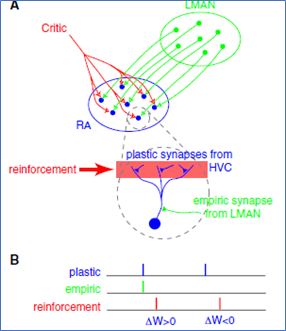
\includegraphics[scale=0.5]{Fiete}
\caption{Fiete's model Roles and learning rule \cite{2}}\label{Fig 2}
A proposal for plasticity rules at HVC\textsubscript{RA} synapses. Synaptic
plasticity rule for gradient estimation by dynamic perturbation of conductance.
We use the actor– critic– experimenter SCHEMA AND distinguish
between plastic and empiric synapses. A: neurons in the experimenter
(LMAN) dynamically perturb the conductance’s of RA neurons through empiric
synapses. Critic signals improvements in performance and globally
broadcasts a reinforcement signal to all plastic synapses (HVC\textsubscript{RA}). B: if
coincident activation of a plastic synapse and empiric synapse onto the same
RA neuron is followed by reinforcement, then the plastic synapse is strengthened.
If activation of the plastic synapse without the empiric synapse is
followed by reinforcement, the plastic synapse is weakened

\end{figure}

The model Fiete suggested at \cite{2} makes some assumptions regarding HVC, RA and LMAN network organization that can guide future research into these specialized areas. One assumption regarding HVC in this model is that the stereotyped sparse behavior observed empirically is fixed throughout time and does not need to be learned. Another point that the model emphasizes is regarding the learning rule. Fiete only provides positive feedback to the neuron using a weak Hebbian rule (see figure 2 above for details). Key takeaway from Fiete’s model are:
\begin{itemize}
    \item Model is more realistic than synaptic feedback since the error and perturbation (experimenter) input are at the neuron level
    \item Model is more realistic than synaptic feedback since the error and perturbation (experimenter) input are at the neuron level
    \item The learning rule holds even is the synapses are embedded in a network that is very complex and independent of parameters choice
    \item The model makes learning harder by:
    \begin{itemize}
        \item Error defined as sum squared error of pitch and amplitude and fed back to the network as 0 or 1 (binarized) if above a certain threshold.
        \item Only positive reinforcement is fed to the network
        \item The adaptive threshold is calculated with a moving window across each moment of the song that goes back over the last few trials. This allows for adapted error that does not fire or not all the time
        \item Varying time delay (temporal imprecision) is used to make learning more difficult and simulate in-vivo observations
        \item Model only used few hundreds HVC and RA neurons. In zebra finch this number is more than 100 time larger
    \end{itemize}
    \item Size of RA does not impact learning speed (number of iteration)
    \item Size of HVC is linear with song duration – no impact on speed of learning
    \item If HVC is not fixed in time, learning speed is linear with HVC size
    \item Model learns song in about 2000 iterations. Zebra finch learns in about 100000
\end{itemize} 
\section{RA modeling}
Research by Leonardo et al. pointed out that the sparse stereotyped activity in HVC give rise to the smooth and continuous muscle input required to produce bird song \cite{4}. Furthermore, Leonardo and Fee \cite{4} suggested a model in which several HVC\textsubscript{RA} neurons connect to a single RA ensemble that produces a song syllable. However, the recordings from RA suggest the opposite – Many RA ensembles are used to activated in fast modulation during bird song motifs and similar acoustic features (like syllables and gaps) in different times during the motif are encoded with different RA ensamples. Researchers \cite{4} suggested that activation in RA is still sparse with each RA ensemble activated during a specific time (about 10 ms long) – See diagram below for RA activation illustration. Note that the integration of different RA muscles into smooth motor signal required for song production occurs at the motor control center (like nXIIts for syrinx (syllable pitch) and respiratory muscles (amplitude) control areas).

\begin{figure}[h!]
\centering
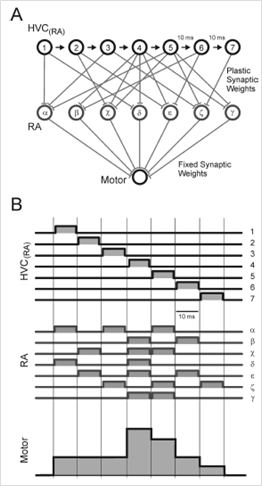
\includegraphics[scale=0.4,center]{Long}
\caption{Leonardo and Fee’s model – Sparse RA activity results in smooth motor activity \cite{4}}\label{Fig 3}
Model of song motor control. A, Working hypothesis for the generation of vocal
control signals. Each HVC\textsubscript{RA} neuron (1–7) bursts at a single time in the song motif. Each of these HVC neurons drives a different subpopulation of RA neurons (α-γ). Activity in RA is then integrated into continuous muscle control signals by the motor unit. Although only one motor output is shown, the model is easily extended to an arbitrary number of outputs. B, Activity patterns in the song motor control model. Discrete and sparse activity in HVC is converted to discrete and dense activity in RA. At each 10 ms time STEPS in the song, a different population of RA neurons is active. In addition, constant vocal outputs can be generated by rapidly evolving patterns of RA activity because of convergence and integration from RA to muscles (time steps 1–3). The end-to-end alignment of burst onsets and offsets is for graphical clarity only; it is not known whether burst patterns in populations of RA or HVC\textsubscript{RA} neurons are organized in this manner.
\end{figure}

\section{HVC Modeling}
The internal HVC structure that give rise to bird song acquisition and production is still a mystery. Research by Long et al. \cite{5} suggested that the HVC contains a structure akin to Synfire chain model that was described by Ables \cite{18} where each unit in one layer is connected to all units in the next layer. Long et al. \cite{5} were able to explain some of the observations in HVC\textsubscript{RA} and internal HVC activity with a simple model using inhibitory HVC interneurons connected in a chain and intrinsic bursting neurons (or in other words, neurons that will fire under normal circumstances unless they are inhibited). The HVC model Long describes at \cite{5} did well to explain how HVC\textsubscript{RA} neuron might work and was robust to noise, jitter in input and other parameters. However, a simple synaptic chain could not explain observations by Glaze et al \cite{19} in which cooling of the HVC produced slowness of the temporal window (e.g. the song became longer) but the gaps (silent period) were lengthen more than the syllable parts of the song in comparison (e.g. a syllable that was 10 ms. long might be 13 ms. long when HVC is cooled, but a silent period during motif that was 10 ms. before cooling could be 15 ms. long after HVC cooling). The cooling and non-uniformed elongation of the song suggests that the synaptic chain model requires adaptation to support the results of \cite{19}. 
In another experiment at Kosche et al \cite{20} were able to show that the stereotyped sparse behavior in HVC\textsubscript{RA} neurons is modulated by interplay of excitatory and inhibitory network within HVC. Specifically, the single activation bout of HVC\textsubscript{RA} neuron was able to activate a network of inhibitory HVC interneurons HVC that in turn caused wide inhibition of other HVC RA neurons. Furthermore, Kosche et al. \cite{20} showed that gaps in activity of the inhibitory interneurons network is necessary to drive the sparse activation of HVC\textsubscript{RA} neurons along with excitatory signal coinciding with the inhibitory gaps. 
Based on Kosche findings \cite{20}, Armstrong et al \cite{21} suggested a Functional Syllable Unit (FSU) for HVC in which each FSU units have two distinct activation modes, one for “quiescence” state and another for winnerless competition state in which the HVC\textsubscript{RA} neurons are activated sequentially. Each FSU unit circuitry has specific connectivity between inhibitory interneurons and excitatory HVC\textsubscript{RA} neurons in the periphery. Armstrong’s model assumes that each FSU will produce only one syllable of short duration and that the sequential activation of FSU units is modulated by feedback signal from the UVA area in the oscine brain. Armstrong’s model addresses some of the findings from \cite{20}, including the high synaptic connectivity between HVC\textsubscript{RA} and HVC interneurons, sequential activation of HVC\textsubscript{RA} units and specific findings regarding current injections into HVC\textsubscript{RA} neurons per \cite{20}. 
\begin{figure}[h]
\centering
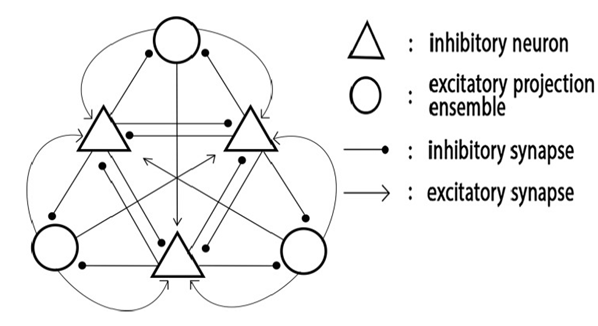
\includegraphics[scale=0.3]{FSU}
\caption{Armstrong's FSU model \cite{21}}\label{Fig 4}
A functional syllable unit (FSU), comprised of 3 inhibitory interneurons (HVC) and 3 ensembles of nucleus (HVC\textsubscript{RA} ) neurons. Triangles and circles represent the former and latter populations, respectively. Circle- and arrow headed lines represent inhibitory and excitatory functional connections, respectively.
\end{figure}
\chapter{Discussion}
Modeling of bird song neural circuitry in HVC and throughout the oscine song system remains an open question. As with other areas of computational neuroscience, models vary in what question / observation they address, methodology used and assumptions. With the advancements in both neuroscience and computational power, the potential for new discoveries on our way to understand how the brain works.
\backmatter
\begin{thebibliography}{22} 
\addcontentsline{toc}{chapter}{\numberline{}Bibliography }
\bibliography{}
\bibitem {1}Nottebohm, F. (2005). The neural basis of birdsong. PLoS biology, 3(5), e164.
\bibitem{2}Fiete, I. R., Fee, M. S., \& Seung, H. S. (2007). Model of birdsong learning based on gradient estimation by dynamic perturbation of neural conductances. Journal of neurophysiology, 98(4), 2038-2057
\bibitem{3} Fiete, I. R., \& Seung, H. S. (2007). Neural network models of birdsong production, learning, and coding. New Encyclopedia of Neuroscience. Eds. L. Squire, T. Albright, F. Bloom, F. Gage, and N. Spitzer. Elsevier
\bibitem{4} Leonardo, A., \& Michale, S. Fee. Ensemble coding of vocal control in birdsong. The Journal of Neuroscience, 25, 652-661.
\bibitem{5} Long, M. A., Jin, D. Z., \& Fee, M. S. (2010). Support for a synaptic chain model of neuronal sequence generation. Nature, 468(7322), 394
\bibitem{6} Aronov, D., Veit, L., Goldberg, J. H., \& Fee, M. S. (2011). Two distinct modes of forebrain circuit dynamics underlie temporal patterning in the vocalizations of young songbirds. Journal of Neuroscience, 31(45), 16353-16368
\bibitem{7}Aronov, D., Andalman, A. S., \& Fee, M. S. (2008). A specialized forebrain circuit for vocal babbling in the juvenile songbird. Science, 320(5876), 630-634.
\bibitem{8}Abbott, L. F., DePasquale, B., \& Memmesheimer, R. M. (2016). Building functional networks of spiking model neurons. Nature neuroscience, 19(3), 350
\bibitem{9}Markowitz, J. E., Liberti III, W. A., Guitchounts, G., Velho, T., Lois, C., \& Gardner, T. J. (2015). Mesoscopic patterns of neural activity support songbird cortical sequences. PLoS biology, 13(6), e1002158.
\bibitem{10}Basista, M. J., Elliott, K. C., Wu, W., Hyson, R. L., Bertram, R., \& Johnson, F. (2014). Independent premotor encoding of the sequence and structure of birdsong in avian cortex. Journal of Neuroscience, 34(50), 16821-16834
\bibitem{11}Brainard, M. S., \& Doupe, A. J. (2002). What songbirds teach us about learning. Nature, 417(6886), 351.
\bibitem{12}Nottebohm, F., Stokes, T. M., \& Leonard, C. M. (1976). Central control of song in the canary, Serinus canarius. Journal of Comparative Neurology, 165(4), 457-486.
\bibitem{13}LeCun, Y., Bengio, Y., \& Hinton, G. (2015). Deep learning. Nature, 521(7553), 436
\bibitem{14}Mooney, R. (2009). Neurobiology of song learning. Current opinion in neurobiology, 19(6), 654-660
\bibitem{15}Orhan, E., \& Ma, W. J. (2018). A Diverse Range of Factors Affect the Nature of Neural Representations Underlying Short-Term Memory. bioRxiv, 244707
\bibitem{16}Brenowitz, E. A., Margoliash, D., \& Nordeen, K. W. (1997). An introduction to birdsong and the avian song system. Journal of neurobiology, 33(5), 495-500
\bibitem{17}Tavanaei, A., Ghodrati, M., Kheradpisheh, S. R., Masquelier, T., \& Maida, A. S. (2018). Deep Learning in Spiking Neural Networks. arXiv preprint arXiv:1804.08150
\bibitem{18}Abeles, M. (2009). Synfire chains. Scholarpedia, 4(7), 1441
\bibitem{19}Glaze, C. M., \& Troyer, T. W. (2006). Temporal structure in zebra finch song: implications for motor coding. Journal of Neuroscience, 26(3), 991-1005
\bibitem{20}Kosche, G., Vallentin, D., \& Long, M. A. (2015). Interplay of inhibition and excitation shapes a premotor neural sequence. Journal of Neuroscience, 35(3), 1217-1227
\bibitem{21}Armstrong, E., \& Abarbanel, H. D. (2016). Model of the songbird nucleus HVC as a network of central pattern generators. Journal of neurophysiology, 116(5), 2405-2419
\bibitem{22}Lenkov, Dmitry N., et al. "Advantages and limitations of brain imaging methods in the research of absence epilepsy in humans and animal models." Journal of neuroscience methods 212.2 (2013): 195-202.
\end{thebibliography}
\end{document}